% Swiss edition plates: painted Nano Banana Pro renders in a Swiss-modern
% register (flat colour blocking, hard edges, no gradients, no outlines, no
% type), replacing the earlier TikZ-drawn plates. Art direction is
% docs/harbor-research/exposition/SWISS-BRIEF.md; the thirteen renders, their
% prompts, and their post-processing are recorded in
% website-v2/public/whitepaper/plates/swiss/PROVENANCE.json. The cover render
% was generated first and then attached as the STYLE TEMPLATE reference to
% every other plate so the thirteen hold together as one set.
%
% \pdswisscoverart draws nothing itself: it makes the cover render the page's
% full-bleed background, leaving the reserved top-left paper for the type the
% TeX sets over it (the cover's title sits at fixed overlay coordinates, so a
% full-bleed image behind it is always safe). \pdswisspartplate{<numeral>}{<width>}
% and \pdswissplate{<prefix>}{<width>} both stay real inline content
% placed after the flowing title/blurb/question text, each at the given
% width and the old TikZ drawing's own aspect (part: 3:2, 24x16 units;
% chapter: 2:1, 24x12 units). There is no drawn fallback: a missing render
% stops the build with a \PackageError naming the missing path.
\makeatletter
\newcommand{\pdswisscoverart}{%
  \IfFileExists{plates/swiss/cover.jpg}{%
    \AddToShipoutPictureBG*{\AtPageLowerLeft{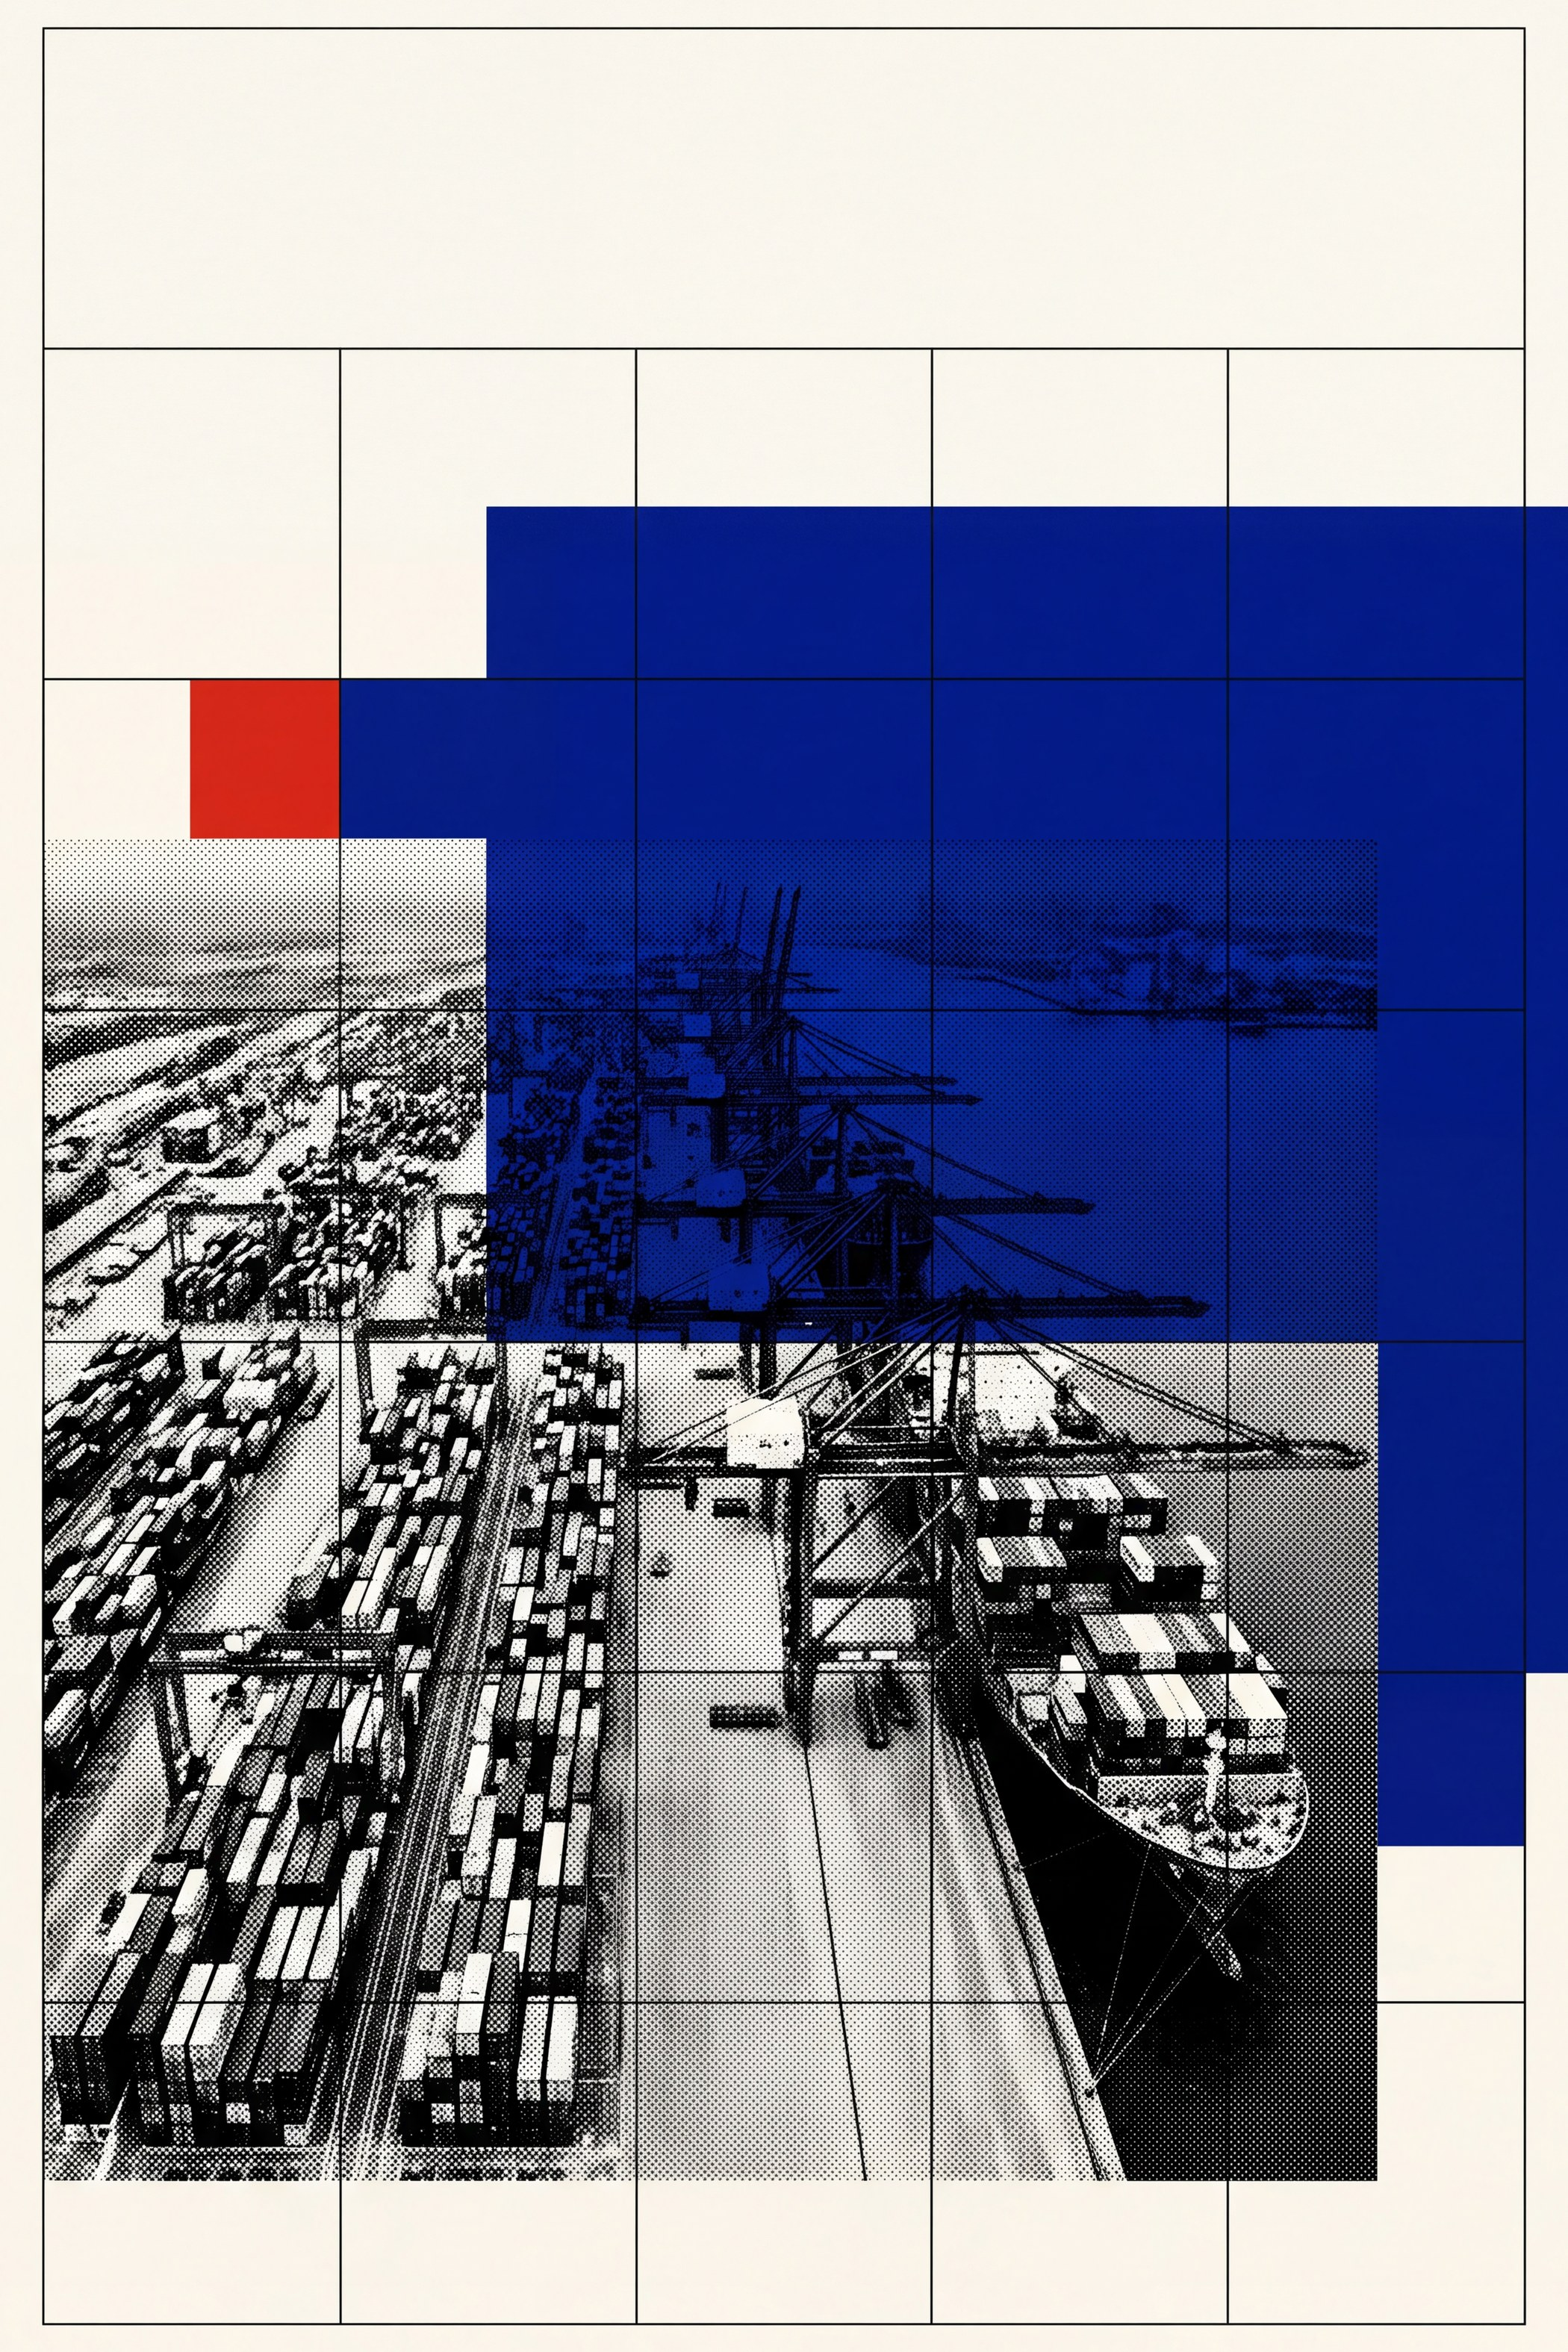
\includegraphics[width=\paperwidth,height=\paperheight]{plates/swiss/cover.jpg}}}}{%
    \PackageError{pd-swiss-plates}{Missing plate render plates/swiss/cover.jpg}{Generate the Swiss cover render and place it at plates/swiss/cover.jpg before building.}}}
\newcommand{\pdswisspartplate}[2]{% #1 numeral I..IV, #2 width
  \IfFileExists{plates/swiss/part-#1.jpg}{%
    \includegraphics[width=#2]{plates/swiss/part-#1.jpg}}{%
    \PackageError{pd-swiss-plates}{Missing plate render plates/swiss/part-#1.jpg}{Generate the Swiss part plate render and place it at plates/swiss/part-#1.jpg before building.}}}
\newcommand{\pdswissplate}[2]{% #1 chapter prefix, #2 width
  \IfFileExists{plates/swiss/chapter-#1.jpg}{%
    \includegraphics[width=#2]{plates/swiss/chapter-#1.jpg}%
  }{%
    \ifstrequal{#1}{prereq}{%
      \IfFileExists{plates/swiss/landmark-01.jpg}{%
        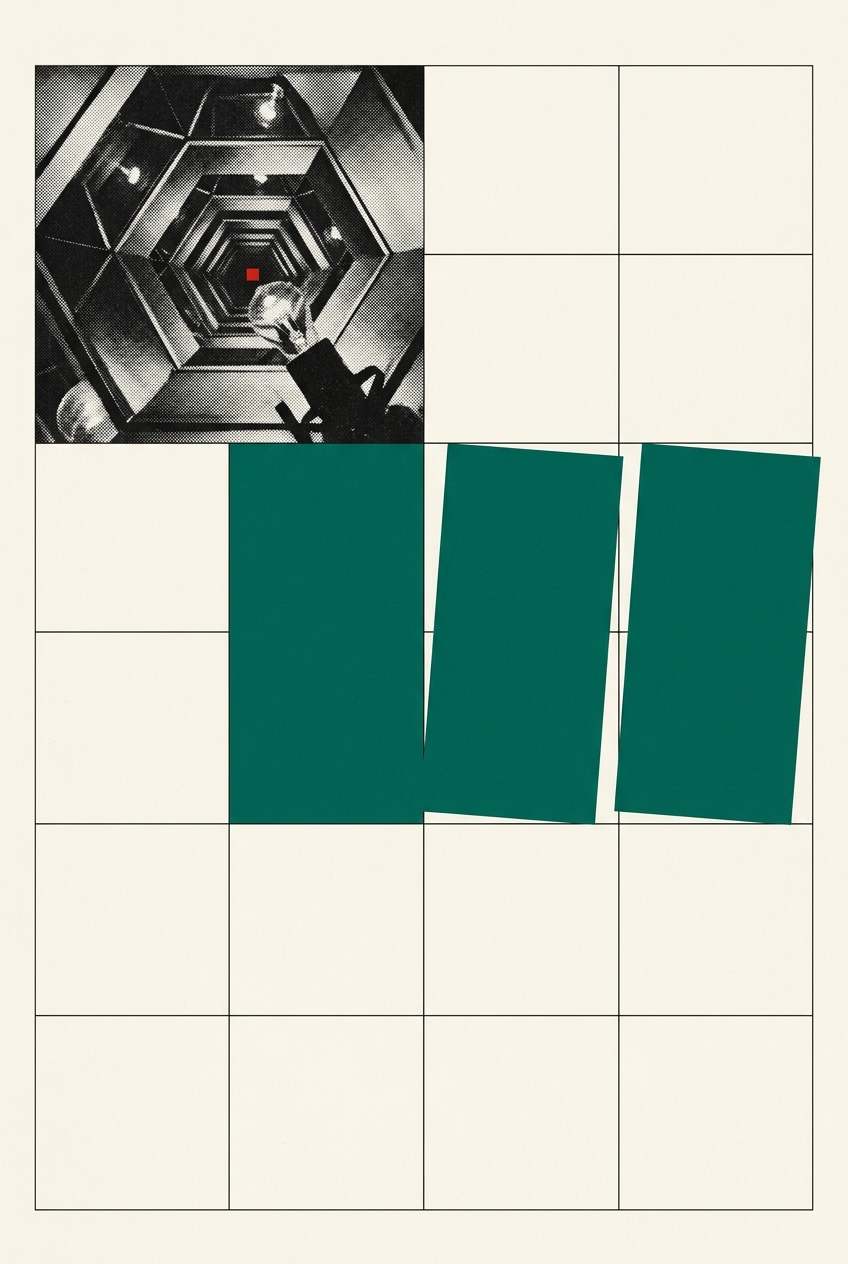
\includegraphics[width=#2]{plates/swiss/landmark-01.jpg}%
      }{%
        \PackageError{pd-swiss-plates}{Missing plate render plates/swiss/landmark-01.jpg}{Generate the Swiss landmark 01 render and place it at plates/swiss/landmark-01.jpg before building.}%
      }%
    }{%
      \PackageError{pd-swiss-plates}{Missing plate render plates/swiss/chapter-#1.jpg}{Generate the Swiss chapter plate render and place it at plates/swiss/chapter-#1.jpg before building.}%
    }%
  }%
}
\providecolor{pdswissred}{HTML}{DA291C}
\providecolor{pdcobalt}{HTML}{001489}
\providecolor{hhink}{HTML}{1B1712}
\providecolor{hhgray}{HTML}{5C5650}

% Canonical Landmark titles and pull-quotes
\expandafter\def\csname pdlandmarktitle@01\endcsname{Agentic Psychosis \& Hallucination Cascade}
\expandafter\def\csname pdlandmarkconcept@01\endcsname{Belief Drift \& Hallucination Cascades}
\expandafter\def\csname pdlandmarkquestion@01\endcsname{Can an unanchored swarm deliberate without spiraling into shared delusion?}
\expandafter\def\csname pdlandmarkquote@01\endcsname{When an unanchored swarm feeds on its own unverified assertions, error does not dissipate; it cascades into conviction. Coordination requires shared physical truth, not mutual agreement on hallucinated state.}

\expandafter\def\csname pdlandmarktitle@02\endcsname{Agentic Continuity \& The Overlapping Strand}
\expandafter\def\csname pdlandmarkconcept@02\endcsname{Substrate Continuity \& Overlapping Strands}
\expandafter\def\csname pdlandmarkquestion@02\endcsname{When every token and worker dies, what actually holds identity across time?}
\expandafter\def\csname pdlandmarkquote@02\endcsname{Identity is not an indivisible core preserved across time, but the continuous overlap of many short fibers. No single thread runs the full length of the rope; the strength is entirely in the friction between the splices.}

\expandafter\def\csname pdlandmarktitle@03\endcsname{The Engine Swap}
\expandafter\def\csname pdlandmarkconcept@03\endcsname{The Engine Swap \& Model Portability}
\expandafter\def\csname pdlandmarkquestion@03\endcsname{Can you replace the brain of a running system while keeping all its commitments intact?}
\expandafter\def\csname pdlandmarkquote@03\endcsname{The intelligence engine may be unbolted and swapped out in mid-voyage. What survives the swap is not the neural weights, but the unbroken hull of contracts, claims, and verified ledger obligations.}

\expandafter\def\csname pdlandmarktitle@04\endcsname{The Front-Loaded Probation Cliff}
\expandafter\def\csname pdlandmarkconcept@04\endcsname{The Front-Loaded Probation Cliff}
\expandafter\def\csname pdlandmarkquestion@04\endcsname{Why should an operating system ever trust an unverified autonomous actor?}
\expandafter\def\csname pdlandmarkquote@04\endcsname{Autonomy is never granted on faith; it is won against a sheer cliff of probation. The newcomer faces strict confinement until its attestation record proves it will not compromise the commons.}

\expandafter\def\csname pdlandmarktitle@05\endcsname{The Single-Writer Monotonic Horizon}
\expandafter\def\csname pdlandmarkconcept@05\endcsname{The Single-Writer Monotonic Horizon}
\expandafter\def\csname pdlandmarkquestion@05\endcsname{How do distributed agents agree on what happened first without Byzantine consensus?}
\expandafter\def\csname pdlandmarkquote@05\endcsname{One writer, one lock, one monotonic frontier. Beyond the commit horizon, the unwritten future remains empty paper; behind it, no write may ever be undone, denied, or reordered.}

\expandafter\def\csname pdlandmarktitle@06\endcsname{The Attenuation Frontier \& Cryptographic Macaroons}
\expandafter\def\csname pdlandmarkconcept@06\endcsname{The Attenuation Frontier \& Macaroons}
\expandafter\def\csname pdlandmarkquestion@06\endcsname{How do permissions travel across machines without accidentally widening?}
\expandafter\def\csname pdlandmarkquote@06\endcsname{Every delegation narrows the aperture of authority. A bearer credential cannot expand its reach as it traverses the network; it can only accumulate cryptographic caveats that bind its hands.}

\expandafter\def\csname pdlandmarktitle@07\endcsname{Attestation Without Revelation (The Sealed Harbor)}
\expandafter\def\csname pdlandmarkconcept@07\endcsname{Attestation Without Revelation (Sealed Harbor)}
\expandafter\def\csname pdlandmarkquestion@07\endcsname{Can a worker prove its computation was correct without revealing what it saw?}
\expandafter\def\csname pdlandmarkquote@07\endcsname{The enclave proves what was computed without disclosing what was seen. Trust in autonomous labor cannot demand total transparency; it demands unforgeable evidence of compliance.}

\expandafter\def\csname pdlandmarktitle@08\endcsname{Read-Poverty \& The Legible Swarm}
\expandafter\def\csname pdlandmarkconcept@08\endcsname{Read-Poverty \& Stigmergic Signaling}
\expandafter\def\csname pdlandmarkquestion@08\endcsname{Why is an agent that reads everything destined to bankrupt its operator?}
\expandafter\def\csname pdlandmarkquote@08\endcsname{In an ocean of synthetic prose, reading is infinitely more expensive than writing. A legible swarm does not shout across channels; it leaves quiet, structured pheromones in the environment.}

\expandafter\def\csname pdlandmarktitle@09\endcsname{Skills as Capital vs.\ Token Labor}
\expandafter\def\csname pdlandmarkconcept@09\endcsname{Skills as Capital vs. Perishable Token Labor}
\expandafter\def\csname pdlandmarkquestion@09\endcsname{When does prompt deliberation become too expensive compared to compiled code?}
\expandafter\def\csname pdlandmarkquote@09\endcsname{Token generation is perishable labor; compiled deterministic tools are durable capital. An economy matures when agents stop paying per token to deliberate and start amortizing proven apparatus.}

\expandafter\def\csname pdlandmarktitle@10\endcsname{The Bonded Commons \& Sacrificial Slashing}
\expandafter\def\csname pdlandmarkconcept@10\endcsname{The Bonded Commons \& Sacrificial Slashing}
\expandafter\def\csname pdlandmarkquestion@10\endcsname{What stops an agent from promising the world and walking away from disaster?}
\expandafter\def\csname pdlandmarkquote@10\endcsname{Trust without collateral is wishful thinking. An agent stakes its bond in the escrow of the commons; when an invariant is breached, the tripwire snaps and the stake is forfeited without appeal.}

\expandafter\def\csname pdlandmarktitle@11\endcsname{Sheaf Laplacian Invariance \& Cycle Consistency}
\expandafter\def\csname pdlandmarkconcept@11\endcsname{Sheaf Laplacians \& Cycle Holonomy}
\expandafter\def\csname pdlandmarkquestion@11\endcsname{Can a network of liars agree locally on every edge while still being caught globally?}
\expandafter\def\csname pdlandmarkquote@11\endcsname{Local consistency along every pairwise edge does not guarantee global truth. When an assertion traverses a closed cycle of harbors and returns altered, the non-zero holonomy reveals the fraud.}

\expandafter\def\csname pdlandmarktitle@12\endcsname{The Zombie Reclaim \& Salvage Graveyard}
\expandafter\def\csname pdlandmarkconcept@12\endcsname{Zombie Salvage \& Dead-Man Leases}
\expandafter\def\csname pdlandmarkquestion@12\endcsname{When an agent crashes in the dark, who buries the body and recovers the locks?}
\expandafter\def\csname pdlandmarkquote@12\endcsname{The graveyard of abandoned sessions is the foundation of harbor resilience. When a heartbeat goes cold, no ghost may linger; the lease expires, the locks are salvaged, and the port is reclaimed.}

% Single-digit alias fallbacks
\expandafter\def\csname pdlandmarktitle@1\endcsname{\csname pdlandmarktitle@01\endcsname}
\expandafter\def\csname pdlandmarkconcept@1\endcsname{\csname pdlandmarkconcept@01\endcsname}
\expandafter\def\csname pdlandmarkquestion@1\endcsname{\csname pdlandmarkquestion@01\endcsname}
\expandafter\def\csname pdlandmarkquote@1\endcsname{\csname pdlandmarkquote@01\endcsname}

\expandafter\def\csname pdlandmarktitle@2\endcsname{\csname pdlandmarktitle@02\endcsname}
\expandafter\def\csname pdlandmarkconcept@2\endcsname{\csname pdlandmarkconcept@02\endcsname}
\expandafter\def\csname pdlandmarkquestion@2\endcsname{\csname pdlandmarkquestion@02\endcsname}
\expandafter\def\csname pdlandmarkquote@2\endcsname{\csname pdlandmarkquote@02\endcsname}

\expandafter\def\csname pdlandmarktitle@3\endcsname{\csname pdlandmarktitle@03\endcsname}
\expandafter\def\csname pdlandmarkconcept@3\endcsname{\csname pdlandmarkconcept@03\endcsname}
\expandafter\def\csname pdlandmarkquestion@3\endcsname{\csname pdlandmarkquestion@03\endcsname}
\expandafter\def\csname pdlandmarkquote@3\endcsname{\csname pdlandmarkquote@03\endcsname}

\expandafter\def\csname pdlandmarktitle@4\endcsname{\csname pdlandmarktitle@04\endcsname}
\expandafter\def\csname pdlandmarkconcept@4\endcsname{\csname pdlandmarkconcept@04\endcsname}
\expandafter\def\csname pdlandmarkquestion@4\endcsname{\csname pdlandmarkquestion@04\endcsname}
\expandafter\def\csname pdlandmarkquote@4\endcsname{\csname pdlandmarkquote@04\endcsname}

\expandafter\def\csname pdlandmarktitle@5\endcsname{\csname pdlandmarktitle@05\endcsname}
\expandafter\def\csname pdlandmarkconcept@5\endcsname{\csname pdlandmarkconcept@05\endcsname}
\expandafter\def\csname pdlandmarkquestion@5\endcsname{\csname pdlandmarkquestion@05\endcsname}
\expandafter\def\csname pdlandmarkquote@5\endcsname{\csname pdlandmarkquote@05\endcsname}

\expandafter\def\csname pdlandmarktitle@6\endcsname{\csname pdlandmarktitle@06\endcsname}
\expandafter\def\csname pdlandmarkconcept@6\endcsname{\csname pdlandmarkconcept@06\endcsname}
\expandafter\def\csname pdlandmarkquestion@6\endcsname{\csname pdlandmarkquestion@06\endcsname}
\expandafter\def\csname pdlandmarkquote@6\endcsname{\csname pdlandmarkquote@06\endcsname}

\expandafter\def\csname pdlandmarktitle@7\endcsname{\csname pdlandmarktitle@07\endcsname}
\expandafter\def\csname pdlandmarkconcept@7\endcsname{\csname pdlandmarkconcept@07\endcsname}
\expandafter\def\csname pdlandmarkquestion@7\endcsname{\csname pdlandmarkquestion@07\endcsname}
\expandafter\def\csname pdlandmarkquote@7\endcsname{\csname pdlandmarkquote@07\endcsname}

\expandafter\def\csname pdlandmarktitle@8\endcsname{\csname pdlandmarktitle@08\endcsname}
\expandafter\def\csname pdlandmarkconcept@8\endcsname{\csname pdlandmarkconcept@08\endcsname}
\expandafter\def\csname pdlandmarkquestion@8\endcsname{\csname pdlandmarkquestion@08\endcsname}
\expandafter\def\csname pdlandmarkquote@8\endcsname{\csname pdlandmarkquote@08\endcsname}

\expandafter\def\csname pdlandmarktitle@9\endcsname{\csname pdlandmarktitle@09\endcsname}
\expandafter\def\csname pdlandmarkconcept@9\endcsname{\csname pdlandmarkconcept@09\endcsname}
\expandafter\def\csname pdlandmarkquestion@9\endcsname{\csname pdlandmarkquestion@09\endcsname}
\expandafter\def\csname pdlandmarkquote@9\endcsname{\csname pdlandmarkquote@09\endcsname}

\newcommand{\pdlandmarktocentry}[2]{%
  \par\addvspace{5pt}\noindent
  \begin{tikzpicture}
    % Background card
    \draw[draw=pdcobalt!25,fill=pdcobalt!2,rounded corners=2pt,line width=0.5pt] (0,0) rectangle (\linewidth, 1.25in);
    \fill[pdcobalt] (0,0) rectangle (3pt, 1.25in);
    
    % Text container
    \node[anchor=north west,inner sep=0pt,text width=0.60\linewidth] at (8pt, 1.25in-6pt) {%
      {\fontsize{8}{10}\selectfont\color{pdcobalt}\bfseries
        Landmark #1\enspace\textperiodcentered\enspace#2}\par\vspace{3pt}%
      \ifcsname pdlandmarkconcept@#1\endcsname
        \colorbox{pdcobalt!10}{\fontsize{6.2}{7.5}\selectfont\bfseries\color{pdcobalt}Governing Concept: \csname pdlandmarkconcept@#1\endcsname}\par\vspace{3pt}%
      \fi
      \ifcsname pdlandmarkquestion@#1\endcsname
        {\fontsize{6}{7.6}\selectfont\itshape\color{hhink}``\csname pdlandmarkquestion@#1\endcsname''}\par\vspace{4pt}%
      \fi
      \tikz[baseline=-2pt]{\draw[draw=pdcobalt,line width=0.9pt,-{Stealth[length=4pt,width=3pt]}] (0,0.08) -- (0.7,0.08) |- (1.5,-0.04);}%
      \enspace{\fontsize{6}{7.2}\selectfont\bfseries\color{pdcobalt}See Plate on page \ifdefined\pdcurrentplatepage\pdcurrentplatepage\fi}%
    };
    
    % Framed thumbnail image on the right
    \node[anchor=north east,inner sep=0pt] at (\linewidth-6pt, 1.25in-6pt) {%
      \fcolorbox{pdcobalt!35}{white}{%
        \includegraphics[width=0.34\linewidth,height=1.13in,keepaspectratio]{plates/swiss/landmark-#1.jpg}%
      }%
    };
  \end{tikzpicture}\par\addvspace{5pt}%
}

\newcommand{\pdswisslandmarkplate}[2]{% #1 landmark ID (e.g. 01..12), #2 width
  \IfFileExists{plates/swiss/landmark-#1.jpg}{%
    \phantomsection\label{landmark:#1}%
    \addcontentsline{toc}{pdplate}{\protect\texorpdfstring{\protect\pdlandmarktocentry{#1}{\csname pdlandmarktitle@#1\endcsname}}{Landmark #1: \csname pdlandmarktitle@#1\endcsname}}%
    \centering
    \includegraphics[width=#2]{plates/swiss/landmark-#1.jpg}%
    \par\vspace{10pt}%
    \begin{minipage}{\linewidth}%
      {\color{pdcobalt}\rule{\linewidth}{1.2pt}}\par\vspace{6pt}%
      \raggedright
      {\color{pdswissred}\rule{4.5pt}{4.5pt}}\enspace%
      {\pdgrotesk\bfseries\scshape\fontsize{9}{11}\selectfont\color{hhink}%
        Landmark #1\enspace\textperiodcentered\enspace\csname pdlandmarktitle@#1\endcsname}\par\vspace{4.5pt}%
      {\pdgrotesk\itshape\fontsize{9.5}{13.5}\selectfont\color{hhink}%
        ``\csname pdlandmarkquote@#1\endcsname''\par}%
      \vspace{6pt}%
      {\color{hhgray!30}\rule{\linewidth}{0.4pt}}%
    \end{minipage}%
  }{%
    \PackageError{pd-swiss-plates}{Missing plate render plates/swiss/landmark-#1.jpg}{Generate the Swiss landmark plate render and place it at plates/swiss/landmark-#1.jpg before building.}}}
\makeatother
